%%%%%%%%%%%%%%%%%%%%%%%%%%%%%%%%%%%%%%%%%%%%%%%%%%%%%%%%%%%%%%%%%%%%%%%%%%%%%%%%%%%%%%%%%%%%%%%%%%%%%%
%
%   Filename    : chapter 4.tex 
%
%   Description : This file will contain your System Model, Algorithm, and Design
%                 
%%%%%%%%%%%%%%%%%%%%%%%%%%%%%%%%%%%%%%%%%%%%%%%%%%%%%%%%%%%%%%%%%%%%%%%%%%%%%%%%%%%%%%%%%%%%%%%%%%%%%%




\chapter{The System Model, Algorithm, and Design}
\label{sec:sysmodel}




\section{System Overview}
The system is a web application that generates communities from data retrieved from Twitter. 
On startup, the user will select an algorithm. Once an algorithm is selected, the user then selects a similarity parameter that is compatible
with the chosen algorithm. Finally, the user chooses to generate communities from the data. The system displays 
the graphical representation of the communities as well as the community evaluation metrics that can be applied 
to the communities based from the chosen algorithm and parameter. The system only has one type of user, which 
can select an algorithm, a parameter, and generate and view communities.




\section{System Objectives}
The system must be able to generate communities using a specific algorithm and similarity parameter. The specific objectives are as follows:




\begin{itemize}
	\item To collect data from Twitter
	\item To clean data collected from the social networks
	\item To detect communities using the supported algorithms and parameters
	\item To display a visualization of the communities
	\item To display the evaluation metrics for the communities
\end{itemize}




\section{System Scope and Limitations}
Data collection is necessary in order to detect the communities from the social network.
Data collected from the social networks will only include the user posts, the follow network (or friend network if from Facebook),
hashtag usage, and mentions.




Cleaning the data is necessary in order to reduce noise in the data as well as to ensure the veracity of the data. This 
would improve the detected communities.




The only algorithms to be considered in the system are divisive and agglomerative hierarchical clustering and fast greedy optimization
of modularity ($FGM$). For the first two algorithms, the only parameters to be considered are the positive/negative valence of posts, 
the subjective/objective valence of posts, the cosine similarity of frequency of topics mentioned, the follow network, hashtag usage,
and mentions.




The visualization is necessary in order to provide a more intuitive representation of the communities. The visualization is limited to 
a graphical visualization to be displayed via HTML5.




Displaying the evaluation metrics is necessary to show the comparative effectiveness of different algorithm and parameter combinations.
The evaluation metrics to be considered are the modularity of the communities and the average mutual following links per user per community
($FPUPC$).








\section{Architectural Design}
The system will follow the MVC architecture. The \texttt{view module} will use HTML5, CSS3, and Javascript. The 
\texttt{controller and model} will be implemented as code.




The \texttt{model module} will include a \texttt{data collection class}, \texttt{representative models} for the data collected, and a \texttt{computational model}.
The UML class diagram for the \texttt{model module} is found in figure \ref{fig:uml}.




\newpage




\begin{landscape}
	\begin{figure}
		\centering
		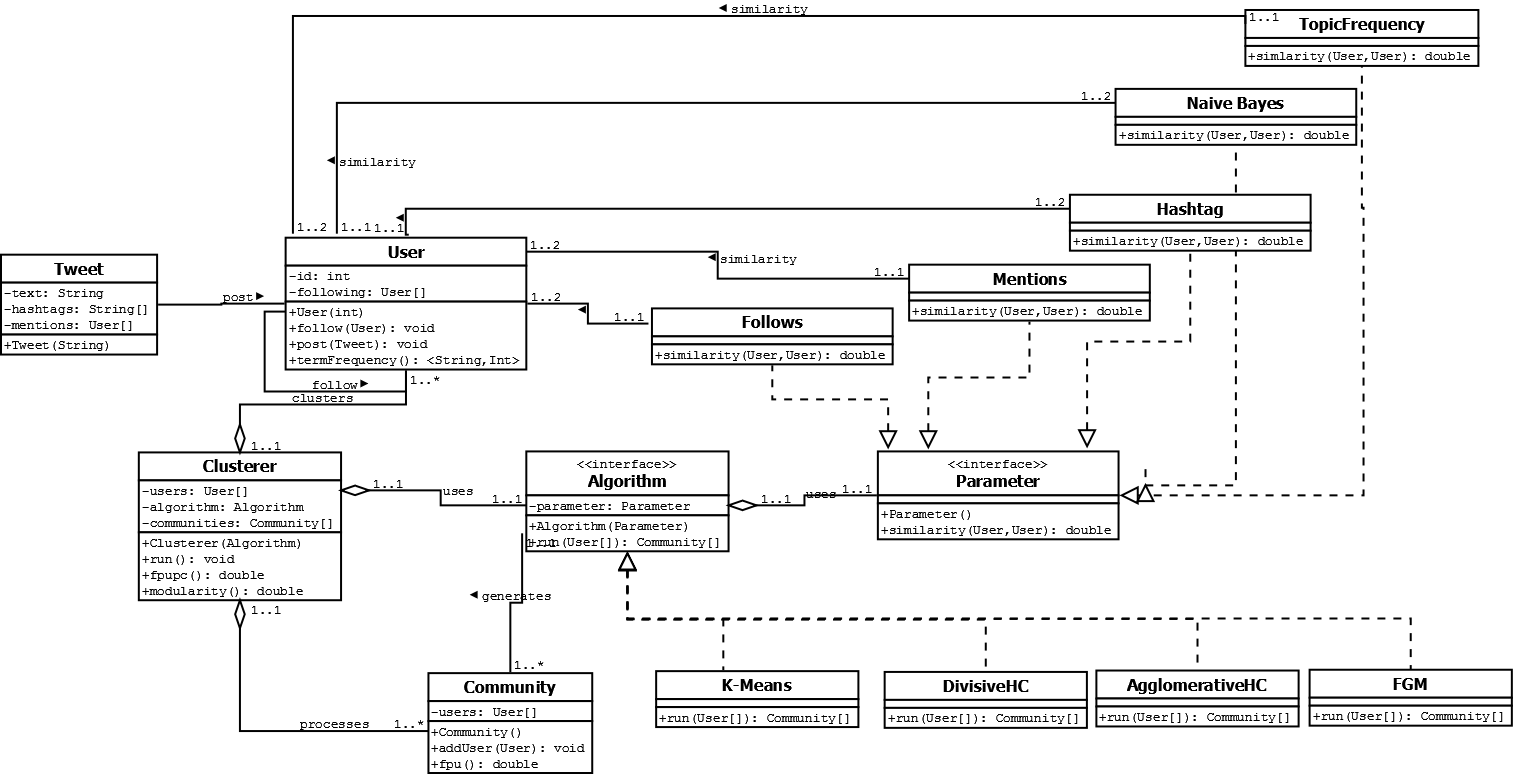
\includegraphics[width=1.4\textwidth]{THS-ST1_FernandezPobleteSanPedroTan_UML_v1}
		\caption{UML Diagram of the Model Component of the Proposed System}
		\label{fig:uml}	
	\end{figure}
\end{landscape}




\newpage




Data collection is done via the \texttt{tweepy} API. The data collection methodology is as follows - a list of user accounts will be specified. This list can be chosen in a way that the users are random, or that the users have some already known relationship which the algorithms will attempt to detect. For each account, their most recent retrievable tweets will be obtained. Next, a breadth-first search (BFS) will be done for that account\vtick s followers, and their most recent tweets will be retrieved as well. 








The \texttt{UserCrawler.py} file has a function \texttt{get\_all\_tweets(usernames, nTweets, max)}, which is responsible for retrieving the most recent \texttt{nTweets} tweets of a list of users, as specified by the \texttt{usernames} parameter. Each of the usernames is initially pushed into a queue. An iterative process then begins, which is described as follows:








At the start of each iteration, a user is popped from the head of the queue. This user’s most recent \texttt{nTweets} tweets are collected, and the list of users, representing the account\vtick s followers, is obtained. For each user in that list, the algorithm checks if it has seen that particular user previously. If not, the user is added to the end of the queue.








This iterative process continues until \texttt{max} total tweets are obtained.








In parallel with the above algorithm, a separate csv file is also generated. This csv file will contain information about the users\vtick following network. Each row of the csv file will begin with the user id of the particular user, followed by the user id\vtick s of all the accounts that user is following.








To anonymize the data, all json elements that may point back to the user are removed. Specifically, these elements are ``name’’, ``description’’, ``profile\_image\_url’’, ``profile\_image\_url\_https’’, ``profile\_background\_image\_url\_https’’, ``profile\_banner\_url’’, and ``profile\_background\_image\_url’’. Additionally, each user id is replaced with an automatically incrementing integer id (starting at 1). This is because the user id can still be mapped to the actual user profile.








For the \texttt{data representation}, this comprises a \texttt{User class} and a \texttt{Tweet class}.




The \texttt{computational model} will have a central class \texttt{Clusterer} which takes a list of users as an attribute, 
as well as an \texttt{Algorithm} object. The algorithm follows the Strategy design pattern, which abstracts the algorithms in
concrete implementations of the \texttt{Algorithm} interface. The \texttt{Algorithm Interface} contains an instance of the \texttt{Parameter interface}
which also follows the Strategy design pattern. In this case, retrieving the similarities between two User objects is abstracted,
to be implemented by the concrete realizations of the Parameter interface. By setting the algorithm and parameter, the \texttt{Clusterer} objects 
runs the algorithm and produces a list of Community objects, which have two derived attributes $modularity$ and $FPUPC$. The \texttt{Clusterer} caches
these Communities and can also return the aggregate $modularity$ and $FPUPC$ of the set of detected communities.




The \texttt{controller} simply interfaces all the model submodules. It checks on startup if the data collection module is done collecting and cleaning data. It passes the data collected, represented as User and Post classes, to the \texttt{Clusterer} class, after setting an algorithm and parameter. This produces the Community objects that the controller then passes as part of the HTTP response.




The \texttt{view module} will be implemented with HTML5, CSS3, and Javascript. 




\section{System Functions}




This section outlines the different functions of the system.




\subsection{Load Users}
\label{us:colldat}




The user prompts the system to collect new data to have a more updated dataset to extract communities from.




Pre-condition: The system is running. (This is automatically run on server startup.)




Scenario:
\begin{enumerate}
\item The user chooses to load users.
\item The user selects a csv file to load.
\item The system displays a progress bar during this process to show the progress of the upload..
\item The system notifies the user that user loading is finished..
\end{enumerate}




Post-condition: The system now has an updated dataset to extract communities from.




Acceptance Criteria:
\begin{itemize}
\item Test if there is stored data. (User story \ref{us:gencom} should output proper communities.)
\item Test if data is clean.
\end{itemize}




\subsection{Select Algorithm}
\label{us:selectalgo}




The user selects an algorithm in order to set a required parameter for generating communities. Figure \ref{fig:selectalgo} shows a sample screen for this user story.


\begin{figure}[h]
	\centering
	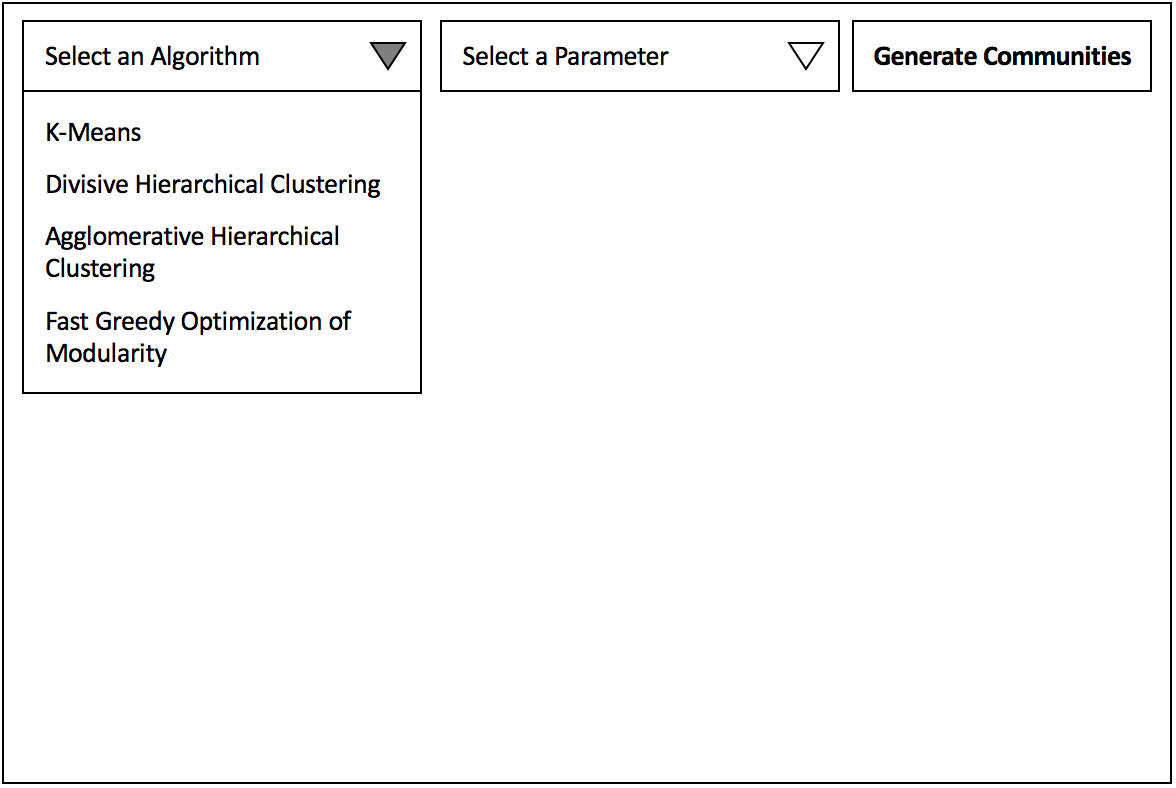
\includegraphics[width=0.5\textwidth]{Mockup_SelectAlgorithm}
	\caption{Sample Screen of User Story \ref{us:selectalgo}}
	\label{fig:selectalgo}	
\end{figure}


Pre-condition: The system has data from Twitter. The main menu is the current screen.




Scenario:
\begin{enumerate}
	\item The user chooses to select an algorithm.
	\item The system displays all the algorithms (K-Means, Divisive Hierarchical Clustering, Agglomerative Hierarchical Clustering, Fast Greedy Optimization of Modularity) supported by the system.
	\item The user selects one of the algorithms.
	\item The user confirms their choice.
	\item The system redirects to the main menu and displays the selected algorithm as part of the system status.
\end{enumerate}




Post-condition: The system has an algorithm to use for generating communities. The ``Select Parameter'' option
is now enabled in the main menu. The allowed parameters have been enabled in the Select Parameter screen.




Acceptance Criteria:
\begin{itemize}
	\item Test if the algorithm selected is valid.
	\item Test if only one algorithm is selected.
	\item Test if the algorithm is displayed as part of the system status.
	\item Test if the system redirects to the main menu.
	\item Test if the ``Select Parameter'' option is now enabled.
\end{itemize}




\subsection{Select Parameter}
\label{us:selectparam}




The user selects a similarity parameter in order to set a required parameter for generating communities. Figure \ref{fig:selectparam} shows a sample screen for this user story.


\begin{figure}[h]
	\centering
	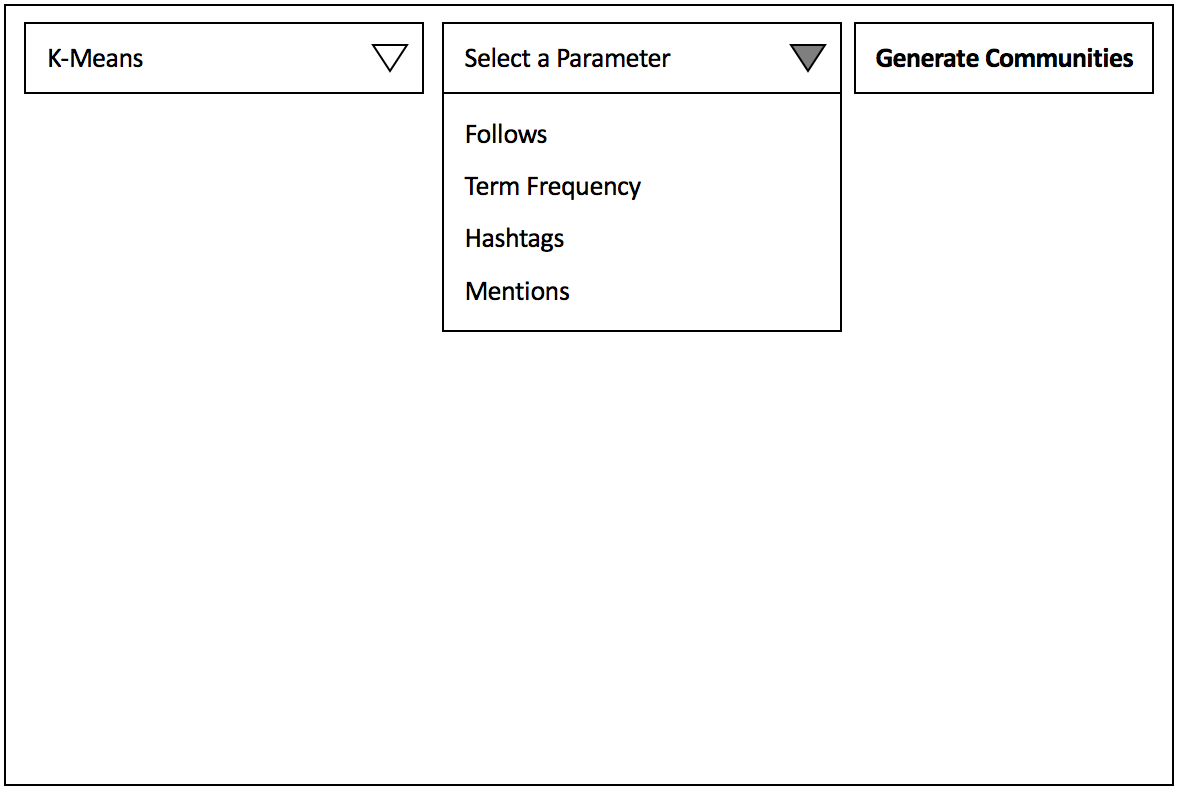
\includegraphics[width=0.5\textwidth]{Mockup_SelectParameter}
	\caption{Sample Screen of User Story \ref{us:selectparam}}
	\label{fig:selectparam}	
\end{figure}




Pre-condition: The system has finished collecting data from the data collection module. User story \ref{us:selectalgo} has been finished.




Scenario:
\begin{enumerate}
	\item The user chooses to select a parameter.
	\item The system displays all parameters compatible with the selected algorithm (Follows, Term Frequency, Hashtags, Mentions).
	\item The user selects one parameter to use.
	\item The user confirms their choice.
	\item The system redirects to the main menu with the ``Generate Communities'' option enabled.
\end{enumerate}




Post-condition: The system has a similarity parameter to use for generating communities. The ``Generate Communities'' option
has been enabled in the main menu.




Acceptance Criteria:
\begin{itemize}
	\item Test if the user has already selected an algorithm.
	\item Test if only the parameters compatible with the selected algorithm are displayed in the ``Select Parameter'' screen.
	\item Test if the parameter selected is a valid choice.
	\item Test if only one parameter is selected.
	\item Test if the system redirects to the main menu.
	\item Test if the ``Generate Communities'' option is enabled.
\end{itemize}




\subsection{Generate Communities}
\label{us:gencom}




The user asks the system to generate communities to see the graphical representation of the communities and to see the 
evaluation metrics of the generated communities for the selected algorithm-parameter combination. Figure \ref{fig:gencom} shows a sample screen for this user story.


\begin{figure}[h]
	\centering
	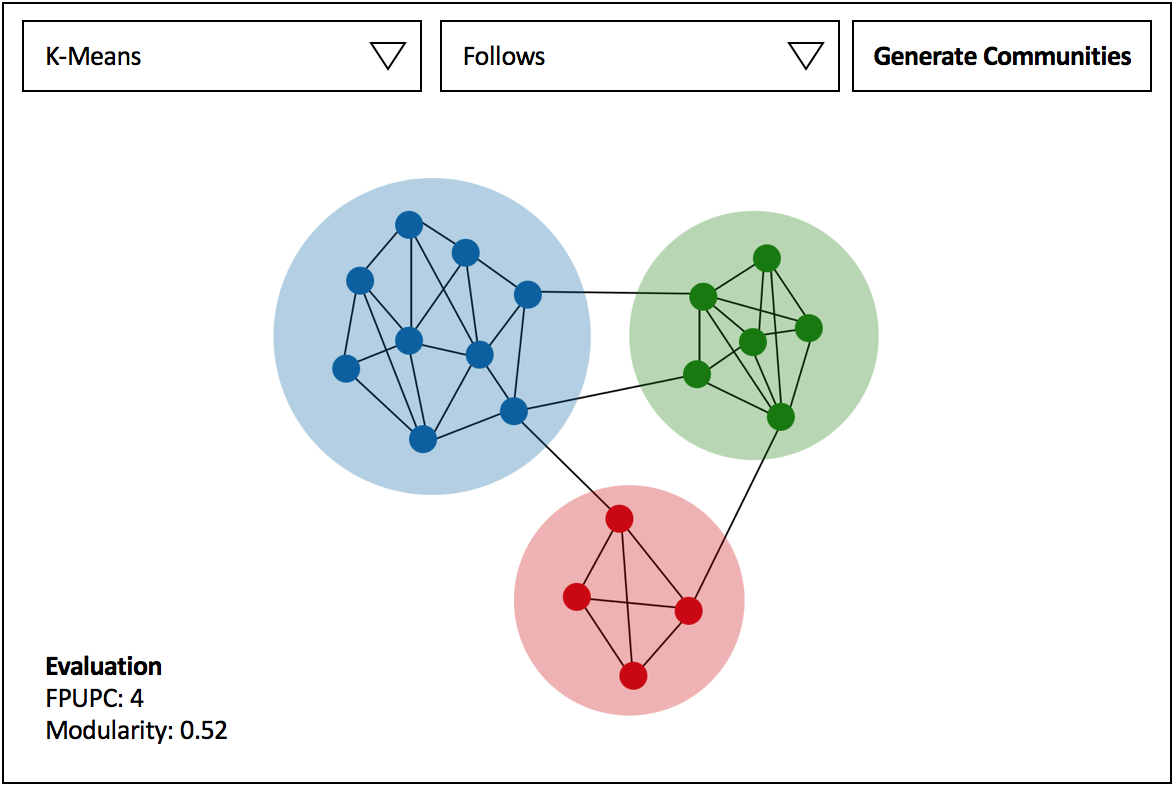
\includegraphics[width=0.5\textwidth]{Mockup_GenerateCommunities}
	\caption{Sample Screen of User Story \ref{us:gencom}}
	\label{fig:gencom}	
\end{figure}


Pre-condition: The system has finished collecting data from the data collection module. User stories \ref{us:selectalgo} and \ref{us:selectparam} have been finished.




Scenario:
\begin{enumerate}
	\item The user chooses to generate communities.
	\item The system computes for the communities using the selected algorithm and parameter.
	\item The system displays the graphical representation of the communities as well as the values of the evaluation metrics.
\end{enumerate}




Post-condition: The system is now displaying a graphical representation of the communities and the value of the evaluation
metrics.




Acceptance Criteria:
\begin{itemize}
	\item Test if the user has already selected an algorithm and parameter.
	\item Test if the detected communities are appropriate for the chosen algorithm and parameter.
	\item Test if the evaluation metrics\vtick values are correct.
\end{itemize}


\subsection{Save Community}
\label{us:savedat}




The user saves a community to be able to do further processing on the community.




Pre-condition: The system is displaying communities.




Scenario:
\begin{enumerate}
\item The user chooses a community.
\item The user selects to save the community.
\item The system displays a progress bar during this process to show the progress of the download.
\item The system notifies the user that the file download is finished.
\end{enumerate}




Post-condition: The user now has a file that can have further processing performed on.




Acceptance Criteria:
\begin{itemize}
\item Test if the file is valid and can be loaded properly
\end{itemize}


\section{Physical Environment and Resources}
The software was developed using Python as a language and Django as a framework for the web application. Python 3.5 is required to run the code. The web application must be run by a server that supports Django 1.10.1. 
